\section{Pressure}
\label{sec:dsmc_pressure}
Pressure plays an important role in the field of fluid flow. An applied pressure difference (which gives a net force) is usually what induces the flow, in addition to being an important property of the fluid. The discussion about pressure contains both how we \textit{define} the pressure, and we \textit{measure} it in a DSMC simulation. And of course how we induce flow in the simulation. It turns out that DSMC satisfies the ideal gas equation of state, so given constant temperature, the local pressure is proportional to the local density. A pressure difference, or pressure gradient, would then require a similar gradient in the density. This is difficult to obtain in a system with periodic boundary conditions because $\rho(x=0) = \rho(x=L)$ for a system of length $L$. Instead we will derive a relation between the pressure gradient and a corresponding constant force which we will use to induce flow in the simulations. 
\subsection{Equation of state}
\label{sec:dsmc_eos}
The free \textit{modules} in a DSMC program are the collision operator $\mathcal C$ and the move operator $\mathcal M$ which fully (stochastically) determine the time evolution of the system. For systems with pairwise interactions (such as hard spheres or the Lennard-Jones potential which we meet in section \ref{sec:md_model}), the pressure may be defined as (see appendix \ref{sec:pressure_derivation} for a derivation)
\begin{align}
	P = \rho_nk_BT + {1\over 3V}\bigg\langle \sum_{i<j} \vec F(\vec r_{ij})\cdot \vec r_{ij}\bigg\rangle,
\end{align}
where the first term is the ideal gas pressure whereas the second term is called the virial of the pressure. Here $\vec F(\vec r_{ij})$ is the force between particle $i$ and $j$, and $\vec r_{ij}$ is their relative distance. In DSMC we don't have the details about the forces, but we can formulate a similar expression using that the force is the change in momentum per time
\begin{align}
	P = \rho_nk_BT + \frac{1}{3Vt}\sum_\text{all collisions} m\Delta \vec v_{ij}\cdot \vec r_{ij},
\end{align}
where $\Delta \vec v_{ij}$ is the change of velocity of one of the particles during a collision\cite{garcia1997direct}. In the collision model we have used, there are no correlation between the change in velocity $\Delta \vec v_{ij}$ and the displacement vector $\vec r_{ij}$ between the particles
\begin{align}
	\left\langle \Delta \vec v_{ij}\cdot \vec r_{ij}\right\rangle = 0,
\end{align}
so the expression for the pressure is reduced to that of an ideal gas
\begin{align}
	P = \rho_n k_BT.
\end{align}
Since the main focus of this thesis is to study dilute gases where the ideal gas is a good approximation, this collision model is sufficient. For dense gases, or liquids, it is possible to apply collision models that yields other equations of state \cite{garcia1997direct}.
\subsection{Measuring pressure}
Since the gas satisfies the ideal gas equation of state, this is of course how we measure the pressure
\begin{align}
	P = \rho_n k_BT,
\end{align}
since we already know how to calculate the density and the temperature. The local pressure is of course found by using the local values of the density and temperature.
\subsection{Applying a pressure gradient}
\label{sec:dsmc_applying_pressured_grad}
In order to induce flow in a system, it is common to apply a pressure gradient. A pressure gradient means that there acts a nonzero net force on any volume element $\dm V$ in the system. In continuum models like the NSE (see section \ref{sec:theory_of_fluids_euler_navier}), the pressure (and hence the pressure gradients) is incorporated as boundary conditions where pressure is specified at given points. A typical boundary condition is $P(x=0) = P_0$ and $P(x=L) = P_L$, but as we already mentioned, periodic boundary conditions is a problem since the points are the very same point. Instead we will use ideas from continuum mechanics to relate a given pressure gradient to a constant force which we will apply on all particles in the system. In the literature, this is often called gravity driven flow.\\
We look at a volume element of size $\Delta V = \Delta x\Delta y\Delta z$ in a channel with a continuous fluid and a pressure gradient in the $x$-direction, see figure \ref{fig:pressure_gravity_equivalent}. 
\begin{figure}[h]
\begin{center}
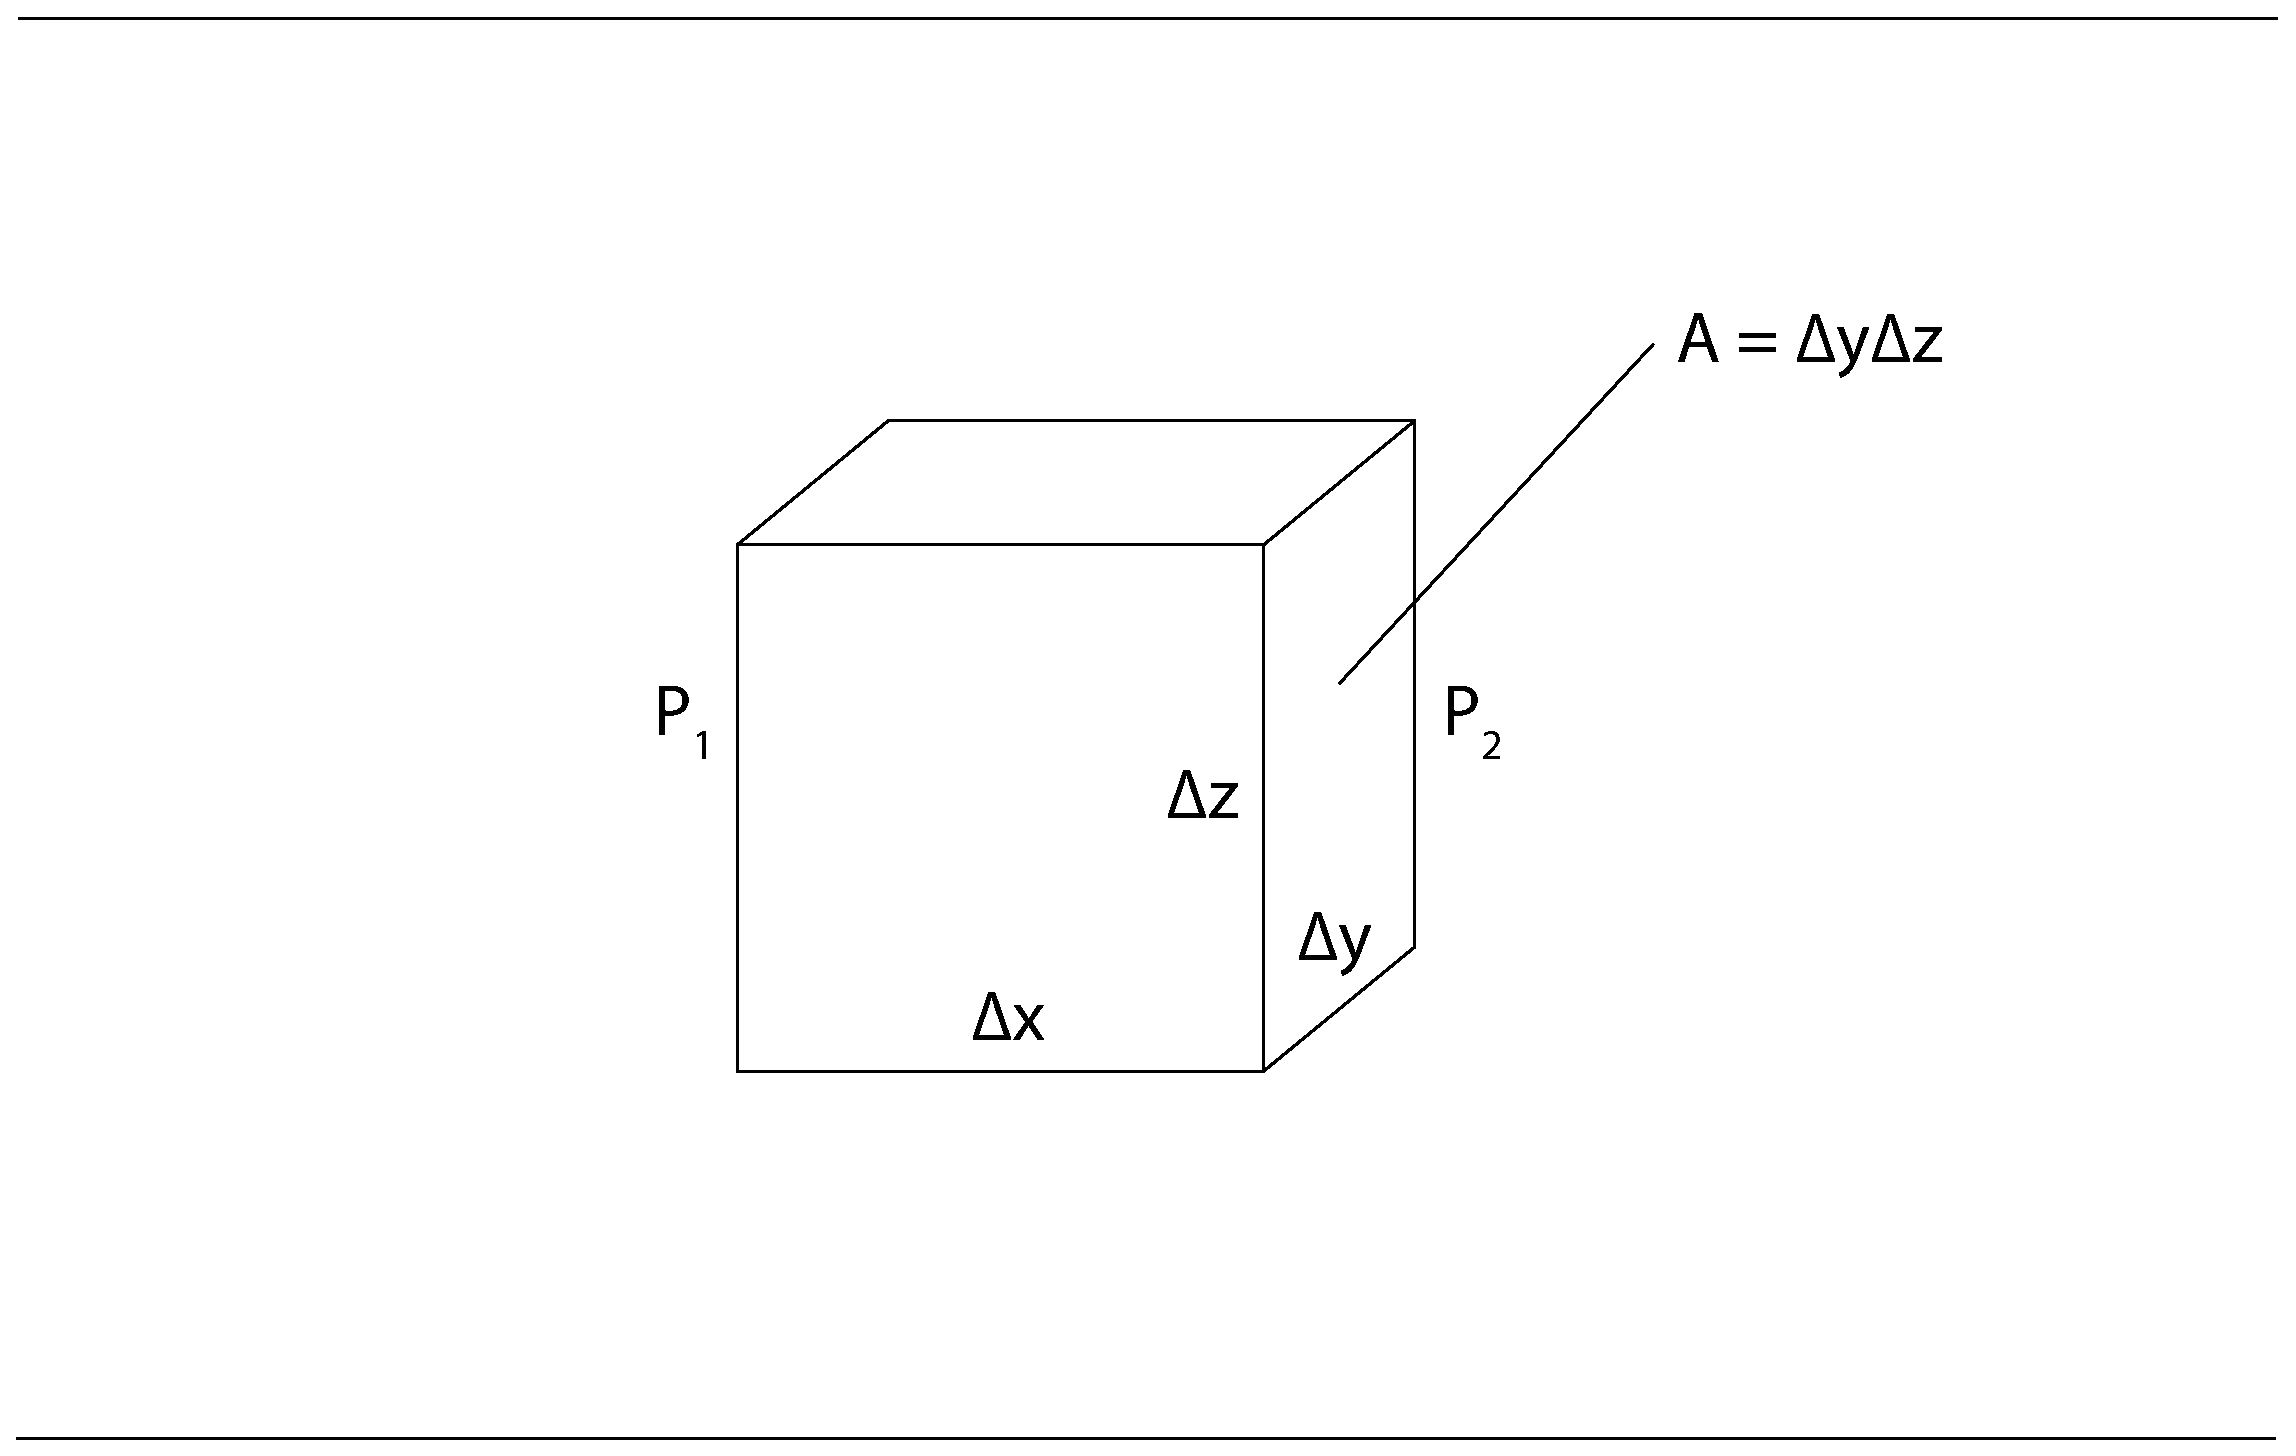
\includegraphics[width=\textwidth, trim=0cm 0cm 0cm 0cm, clip]{DSMC/figures/pressure_to_gravity.eps}
\end{center}
\caption{The net force acting on the volume element $\Delta V = \Delta x\Delta y\Delta z$ in the $x-$direction is given by the pressure difference times area $A(P_2 - P_1) = \Delta y\Delta z\Delta P$.}
\label{fig:pressure_gravity_equivalent}
\end{figure}
The net force acting on the volume element in the $x-$direction is
\begin{align}
	F = P_2\Delta y\Delta z - P_1\Delta y\Delta z = \Delta y\Delta z\Delta P,
\end{align}
where $\Delta P = P_2 - P_1$. We aim to find a constant force $F=mg$ being equivalent to that of the pressure difference. Given an acceleration $g$, the force is then
\begin{align}
	F = mg = \rho_m \Delta V g.
\end{align}
We aim to find a force equal to the one from the pressure difference
\begin{align}
	F = \Delta y\Delta z\Delta P = \Delta V \frac{\Delta P}{\Delta x},	
\end{align}
which gives the relation
\begin{align}
	\label{eq:acceleration_to_pressure_difference}
	g = \frac{\Delta P}{\rho_m\Delta x}.
\end{align}
In simple geometries like a tube, the behavior of the flow for both pressure models should be similar. However, for disordered systems with regions that can \textit{trap} particles, we can expect some effects that will affect the fluid flow in a non-physical way. An example is shown in figure \ref{fig:gravity_problem} where a gas driven by a constant acceleration in the x-direction will be slowed down in the area marked gray. In a gas driven by a real pressure difference, we expect a net force along the channel in all regions.
\begin{figure}[h]
\begin{center}
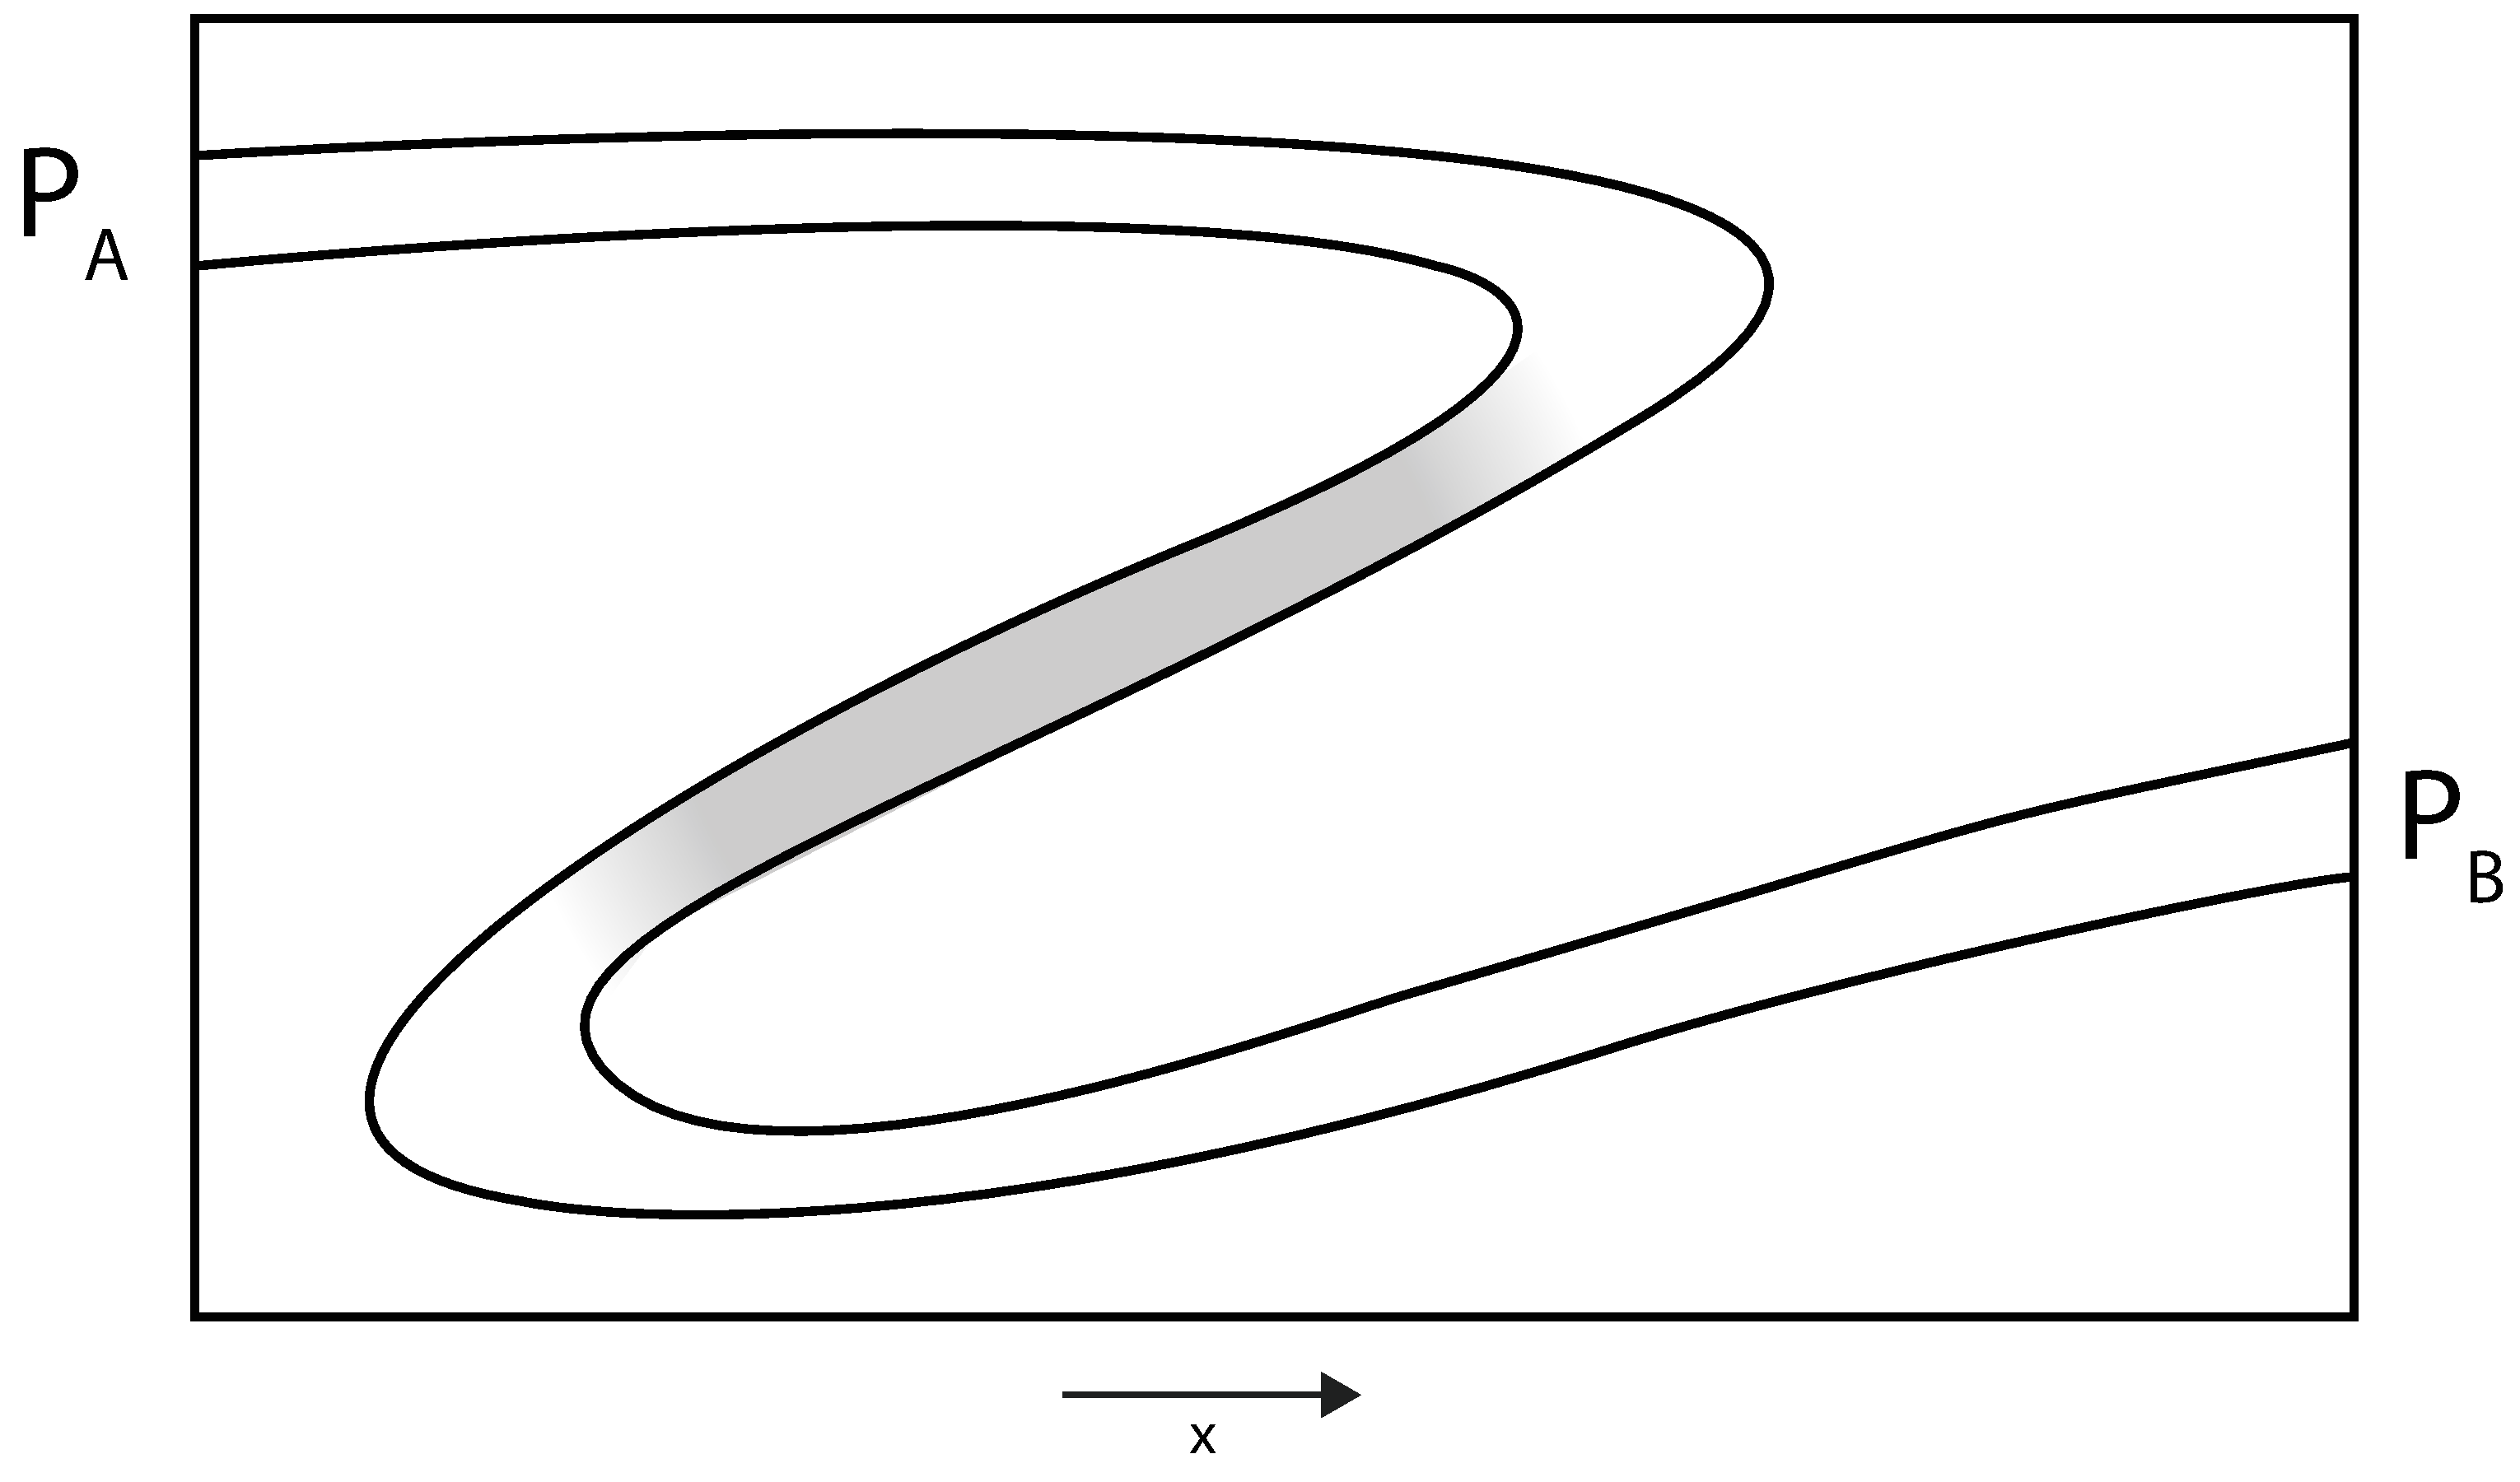
\includegraphics[width=0.7\textwidth, trim=0cm 0cm 0cm 0cm, clip]{DSMC/figures/gravity_problem.eps}
\end{center}
\caption{Flow induced by a constant acceleration will not reproduce correct flow behavior when the gas in a larger part (marked gray) of the channel flows in the opposite direction of the force. In a \textit{real} pressure-driven flow, the net force on the gas will point along the expected flow direction, also in the gray marked area, whereas the acceleration-driven flow will be slowed down.}
\label{fig:gravity_problem}
\end{figure}
\\
We can now obtain a desired pressure difference through equation \eqref{eq:acceleration_to_pressure_difference} and apply that acceleration to all particles each timestep.